\documentclass[a0paper,portrait]{baposter}
\usepackage{lmodern}
\usepackage[utf8]{inputenc} %unicode support
\usepackage[T1]{fontenc}
\usepackage{geometry}
\usepackage{amsmath,amssymb}
\selectcolormodel{cmyk}
\usepackage{relsize}% For \smaller
\usepackage{url}% For \url
\usepackage{epstopdf}	
\usepackage{amsmath}
\usepackage{multicol}
\setlength{\columnsep}{0.1 em}

\usepackage{graphicx}
\usepackage{tcolorbox}
\usepackage{wrapfig}
\graphicspath{{figures/}} % Directory in which figures are stored
\newcommand{\compresslist}{%
\setlength{\itemsep}{0pt}%
\setlength{\parskip}{1pt}%
\setlength{\parsep}{0pt}%
}
\newenvironment{boenumerate}
  {\begin{enumerate}\renewcommand\labelenumi{\textbf\theenumi.}}
  {\end{enumerate}}
\begin{document}
%\definecolor{darkgreen}{cmyk}{0.14,0.13,0.8,0.18}
%\definecolor{lightblue}{cmyk}{0.8,0,0.8,0.25}
\begin{poster}
{
grid=false,
headerborder=open, % Adds a border around the header of content boxes
colspacing=0.5em, % Column spacing
bgColorOne=white, % Background color for the gradient on the left side of the poster
bgColorTwo=white, % Background color for the gradient on the right side of the poster
borderColor=black, % Border color
headerColorOne=black, % Background color for the header in the content boxes (left side)
headerColorTwo=black, % Background color for the header in the content boxes (right side)
headerFontColor=white, % Text color for the header text in the content boxes
boxColorOne=white, % Background color of the content boxes
textborder=rounded, %rectangle, % Format of the border around content boxes, can be: none, bars, coils, triangles, rectangle, rounded, roundedsmall, roundedright or faded
eyecatcher=true, % Set to false for ignoring the left logo in the title and move the title left
headerheight=0.11\textheight, % Height of the header
headershape=rounded, % Specify the rounded corner in the content box headers, can be: rectangle, small-rounded, roundedright, roundedleft or rounded
headershade=plain,
headerfont=\Large\textsf, % Large, bold and sans serif font in the headers of content boxes
%textfont={\setlength{\parindent}{1.5em}}, % Uncomment for paragraph indentation
linewidth=2pt % Width of the border lines around content boxes
}
{}
%
%
{
\textsf %Sans Serif
{Energy landscapes of the designed protein Top7 and some trefoil knots}
}
{\sf
Sridhar Neelamraju$\dagger$ $\ddagger$, Shachi Gosavi$\dagger$ and David J. Wales$\ddagger$ 
\small{\\$\dagger$National Centre for Biological Sciences, Bangalore, India $\ddagger$ University Chemical Laboratories, Lensfield Road, University of Cambridge, UK.}}{
\includegraphics[width=3.5in]{logo.pdf}}

\headerbox{1. Introduction}{name=introduction,column=0,row=0, span=2}{Proteins designed artificially have not had the benefit of evolution and are typically designed only to stabilise the native state. Natural proteins, on the other hand, have evolved to function as well as fold in a minimally frustrated manner. Thus, potential energy landscapes (PELs) of designed proteins are likely to contain topological traps. Here, we study the potential energy landscapes of Top7, a model designed protein and S6, a natural protein of comparable size, using a combination of molecular dynamics (MD) and discrete path sampling (DPS)[1]. Possible kinetic traps and the energetic barriers separating them from the native state are elucidated. We quantify topological frustration resulting from the designed topology of Top7 with a frustration density parameter[2]. Topological frustration is also  evident in knotted proteins. Thus, we extend this methodology to locate topological traps on the PEL of two model trefoil knotted proteins.}
\headerbox{2. Structure Based Models}{name=gokit,column=0,below=introduction,span=2}
{
\begin{equation}
\small
\begin{aligned}
U = &
\sum_{i=1,N-1}\frac{K_b}{2}\big(r_i-r_O\big) + \sum_{i=1,N-2}K{_\theta} \big( \theta _i - \theta_O\big )  + \sum_{i=1,N-3}\frac{K_{\phi}}{2}\big( 1-cos\big( 2\phi_i - \frac{\pi}{2}\big)\big) \\ 
   & +\sum_{i<j-3}^{Nat-C}\epsilon_{ij}\Big[5\Big( \frac{\sigma_{ij}}{r_{ij}}\Big)^{12} - 6\Big( \frac{\sigma_{ij}}{r_{ij}}\Big)^{10}  \Big] + \sum_{i<j-3}^{Non-C}\epsilon_{ij}\Big(\frac{C}{r_{ij}}\Big)^{12}
\label{eq:eq1}
\end{aligned}
\end{equation}
Artificial frustration is added by introducing non-native attractive interactions among hydrophobic residues. 
Effect of intercalated water molecules is approximated by a desolvation barrier potential. Effect of side-chain interactions with a statistical two-bead Cheung-Thirumalai potential. See ``Go-kit''[3] for list of models implemented and application of these models to single domain proteins with Discrete Path Sampling and Molecular Dynamics.}

\headerbox{3. Visualising the energy landscape}{name=Top7,column=2, span=1, row=0}{ 
\begin{center}
 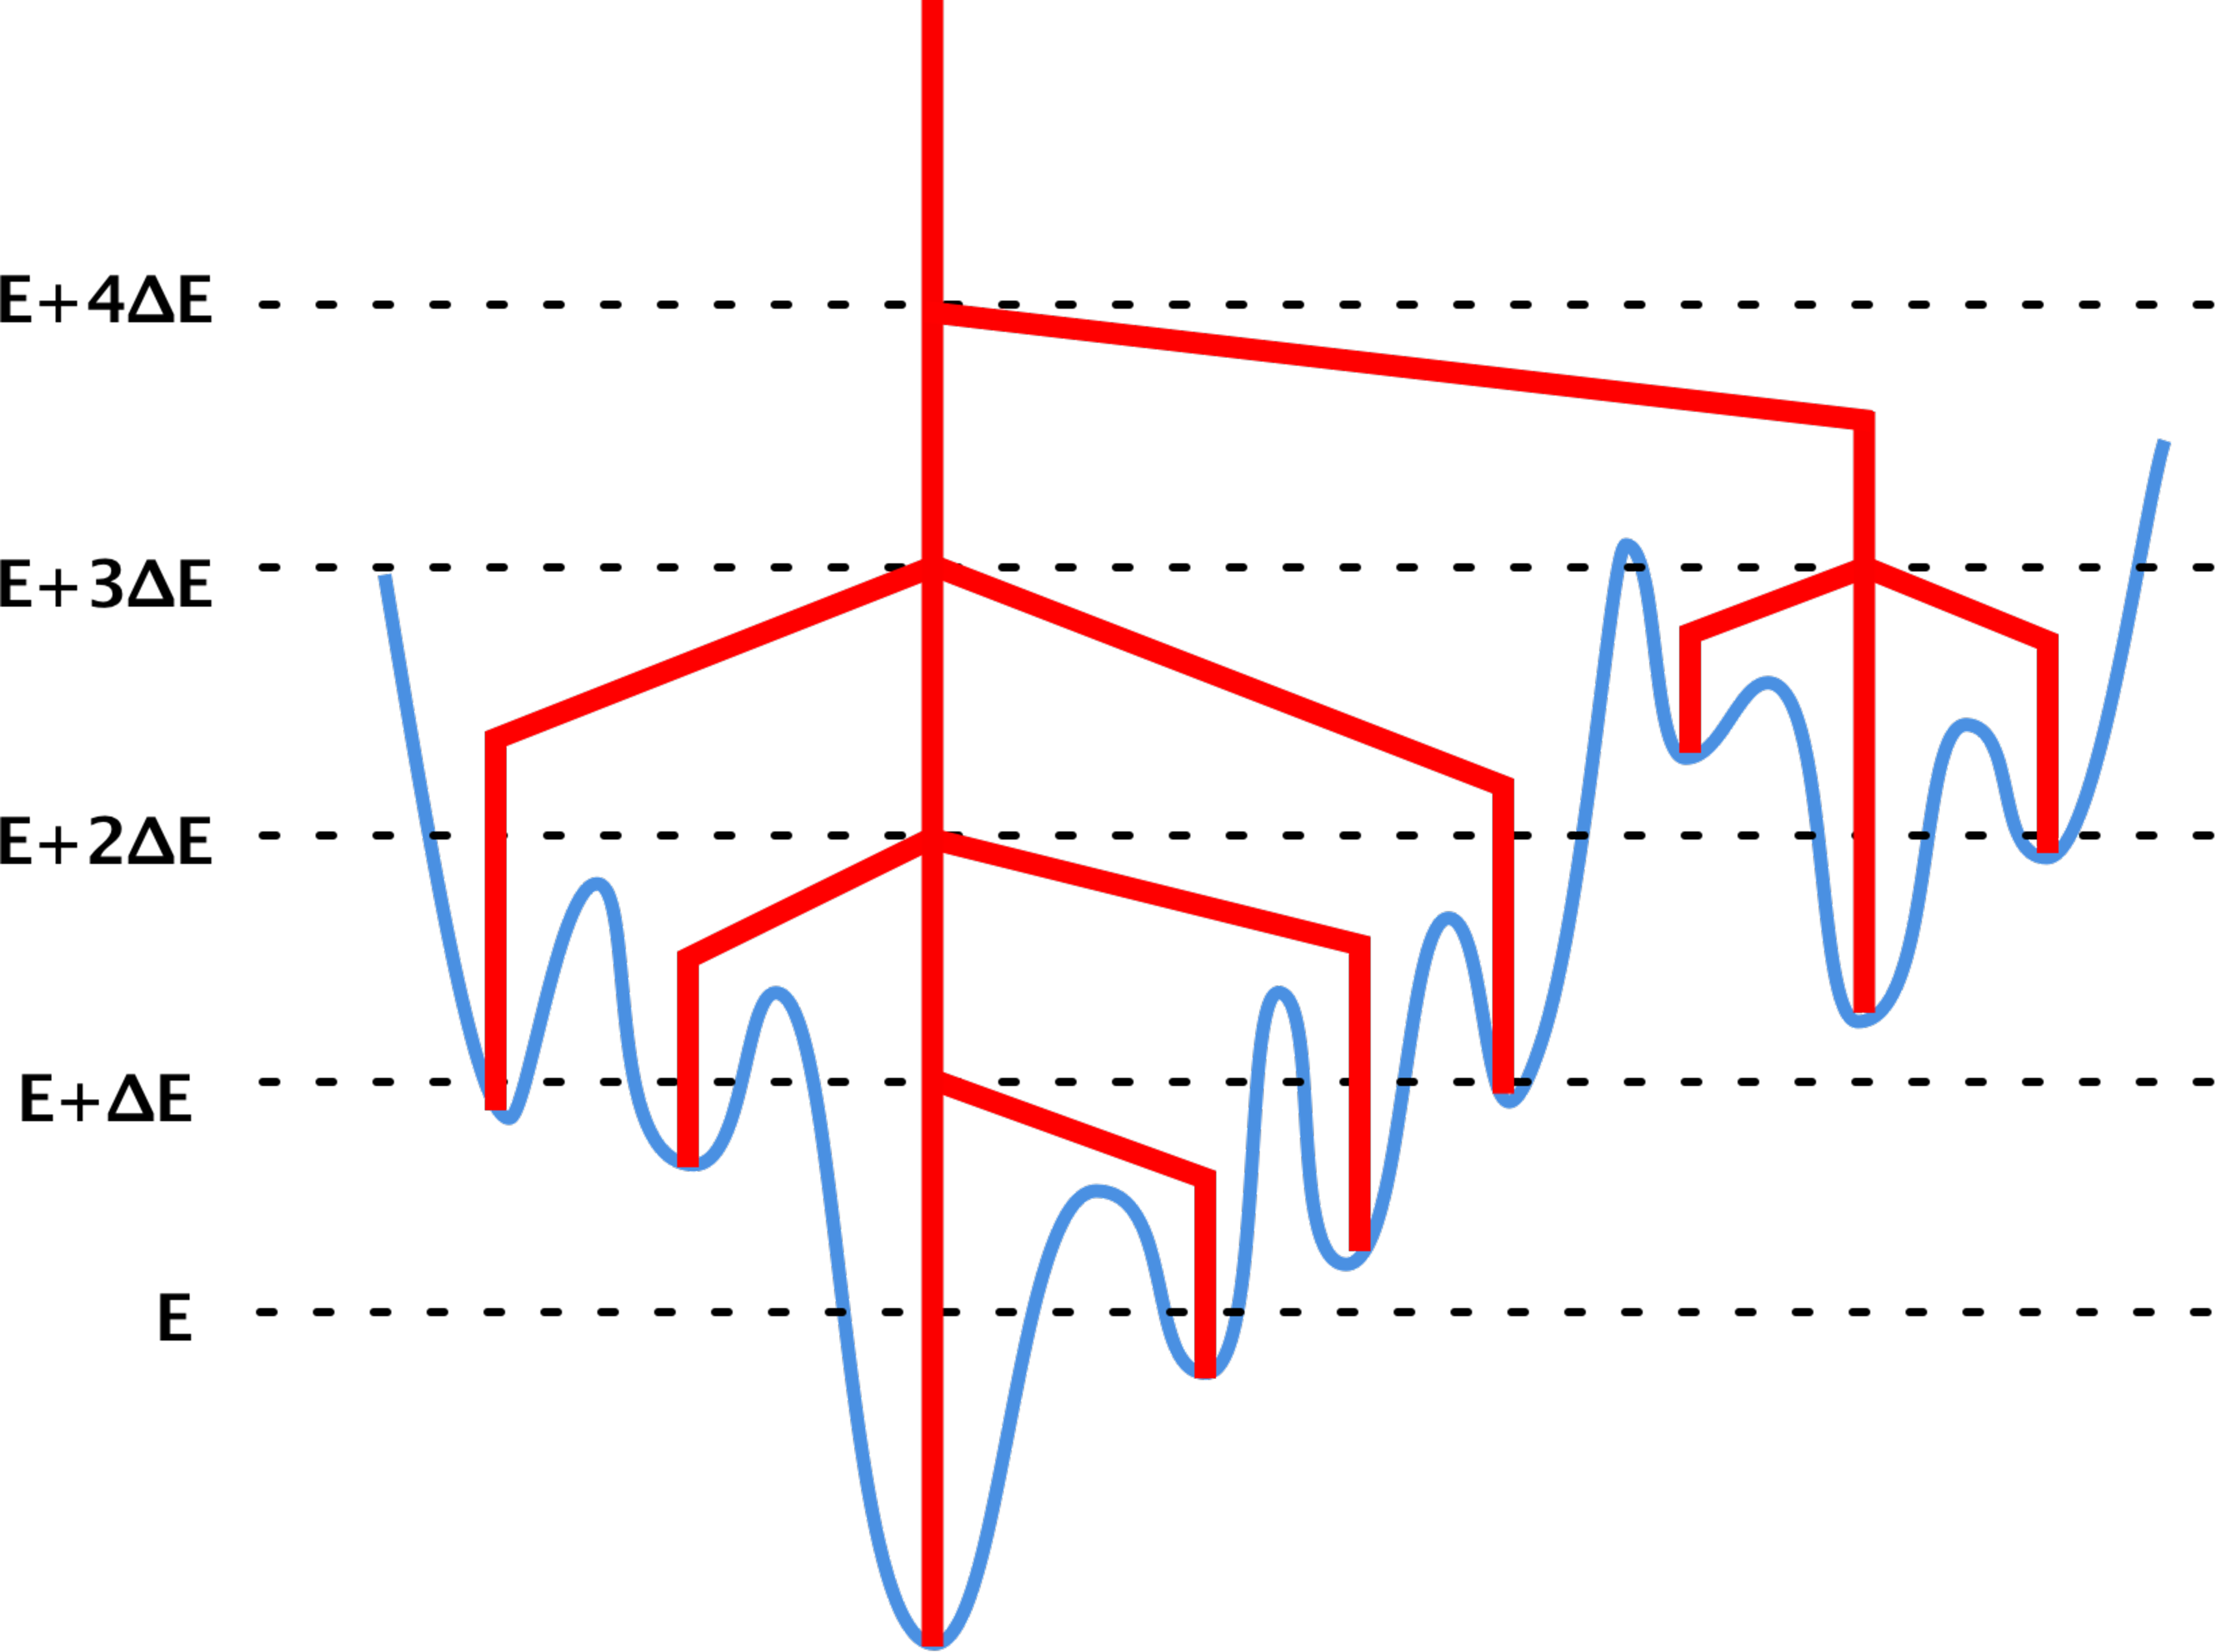
\includegraphics[width=0.6\linewidth]{disconn.pdf}
\end{center}
\vspace{-0.4cm}
The PEL is visualised as a microcanonical disconnectivity graph[4]. Each minimum corresponds to a vertical branch terminating at the corresponding potential energy. For a regular series of threshold energies spaced by a chosen value, $\Delta$E, a superbasin analysis is performed to separate the minima into disjoint sets, whose members can interconvert without exceeding a transition state energy above the current threshold. The branches join at nodes on the vertical (energy) axis as the superbasins merge. A fully funneled landscape is characterised by a ``Palm Tree'' like appearance. 
}

\headerbox{4. Top7:Discrete Path Sampling}{name=Top7DPS,column=0, span=1, below=gokit}{ % To reduce this block to 1 column width, remove 'span=2'
\begin{center}
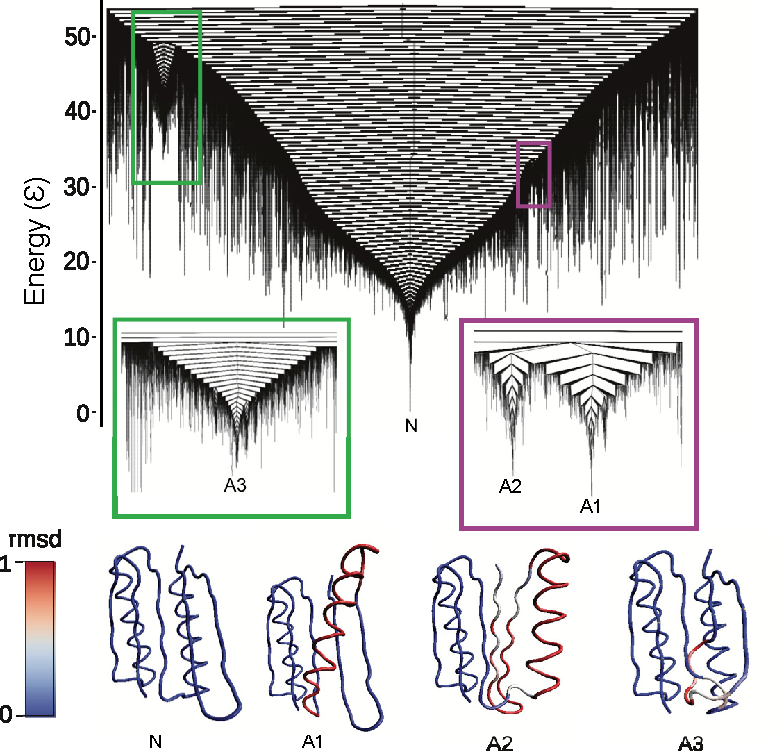
\includegraphics[width=0.8\linewidth]{tree4_5.pdf} \\   
\end{center}
Disconnectivity graph representation of the ensemble of stationary points derived with DPS for Top7 (C$\alpha$, 4.5 \AA). Blue indicates the parts of the protein similar to the native state (N) and red indicates the RMSD difference from N. A1, A2 and A3 are kinetic traps found on the potential energy landscape.\\}


\headerbox{5. Top7 Vs S6: Frustration Density}{name=Top7frust,column=1, span=1, below=gokit}{ % To reduce this block to 1 column width, remove 'span=2'
\begin{center}
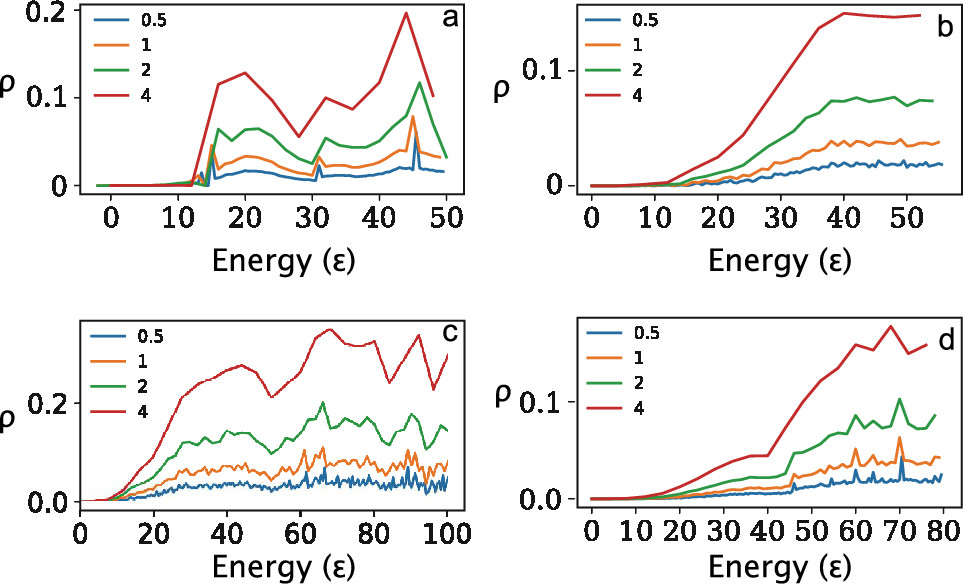
\includegraphics[width=\linewidth]{frustrationdensity.jpeg} \\
\end{center}
Frustration density, $\rho$, as a function of the energy interval for disconnectivity graphs at $\delta$=0.5$\varepsilon$ (blue), 1$\varepsilon$ (orange), 2$\varepsilon$ (green) and 4$\varepsilon$ (red). (a) Top7 - C$\alpha$ model (b) S6 - C$\alpha$ model (c) Top7 - C$\alpha$-C$\beta$ model and (d) M7- C$\alpha$ model. The horizontal axis is scaled to $\delta$=1$\varepsilon$. For Top7, the SBM representation shows distinct fluctuation in the frustration density parameter. For S6, and M7 (a cooperatively folding protein designed to fold into the topology of Top7), the fluctuations are absent.}

\headerbox{6. Probability contact map: Top7}{name=PCM,column=2, span=1, below=Top7}{ 
\begin{center}
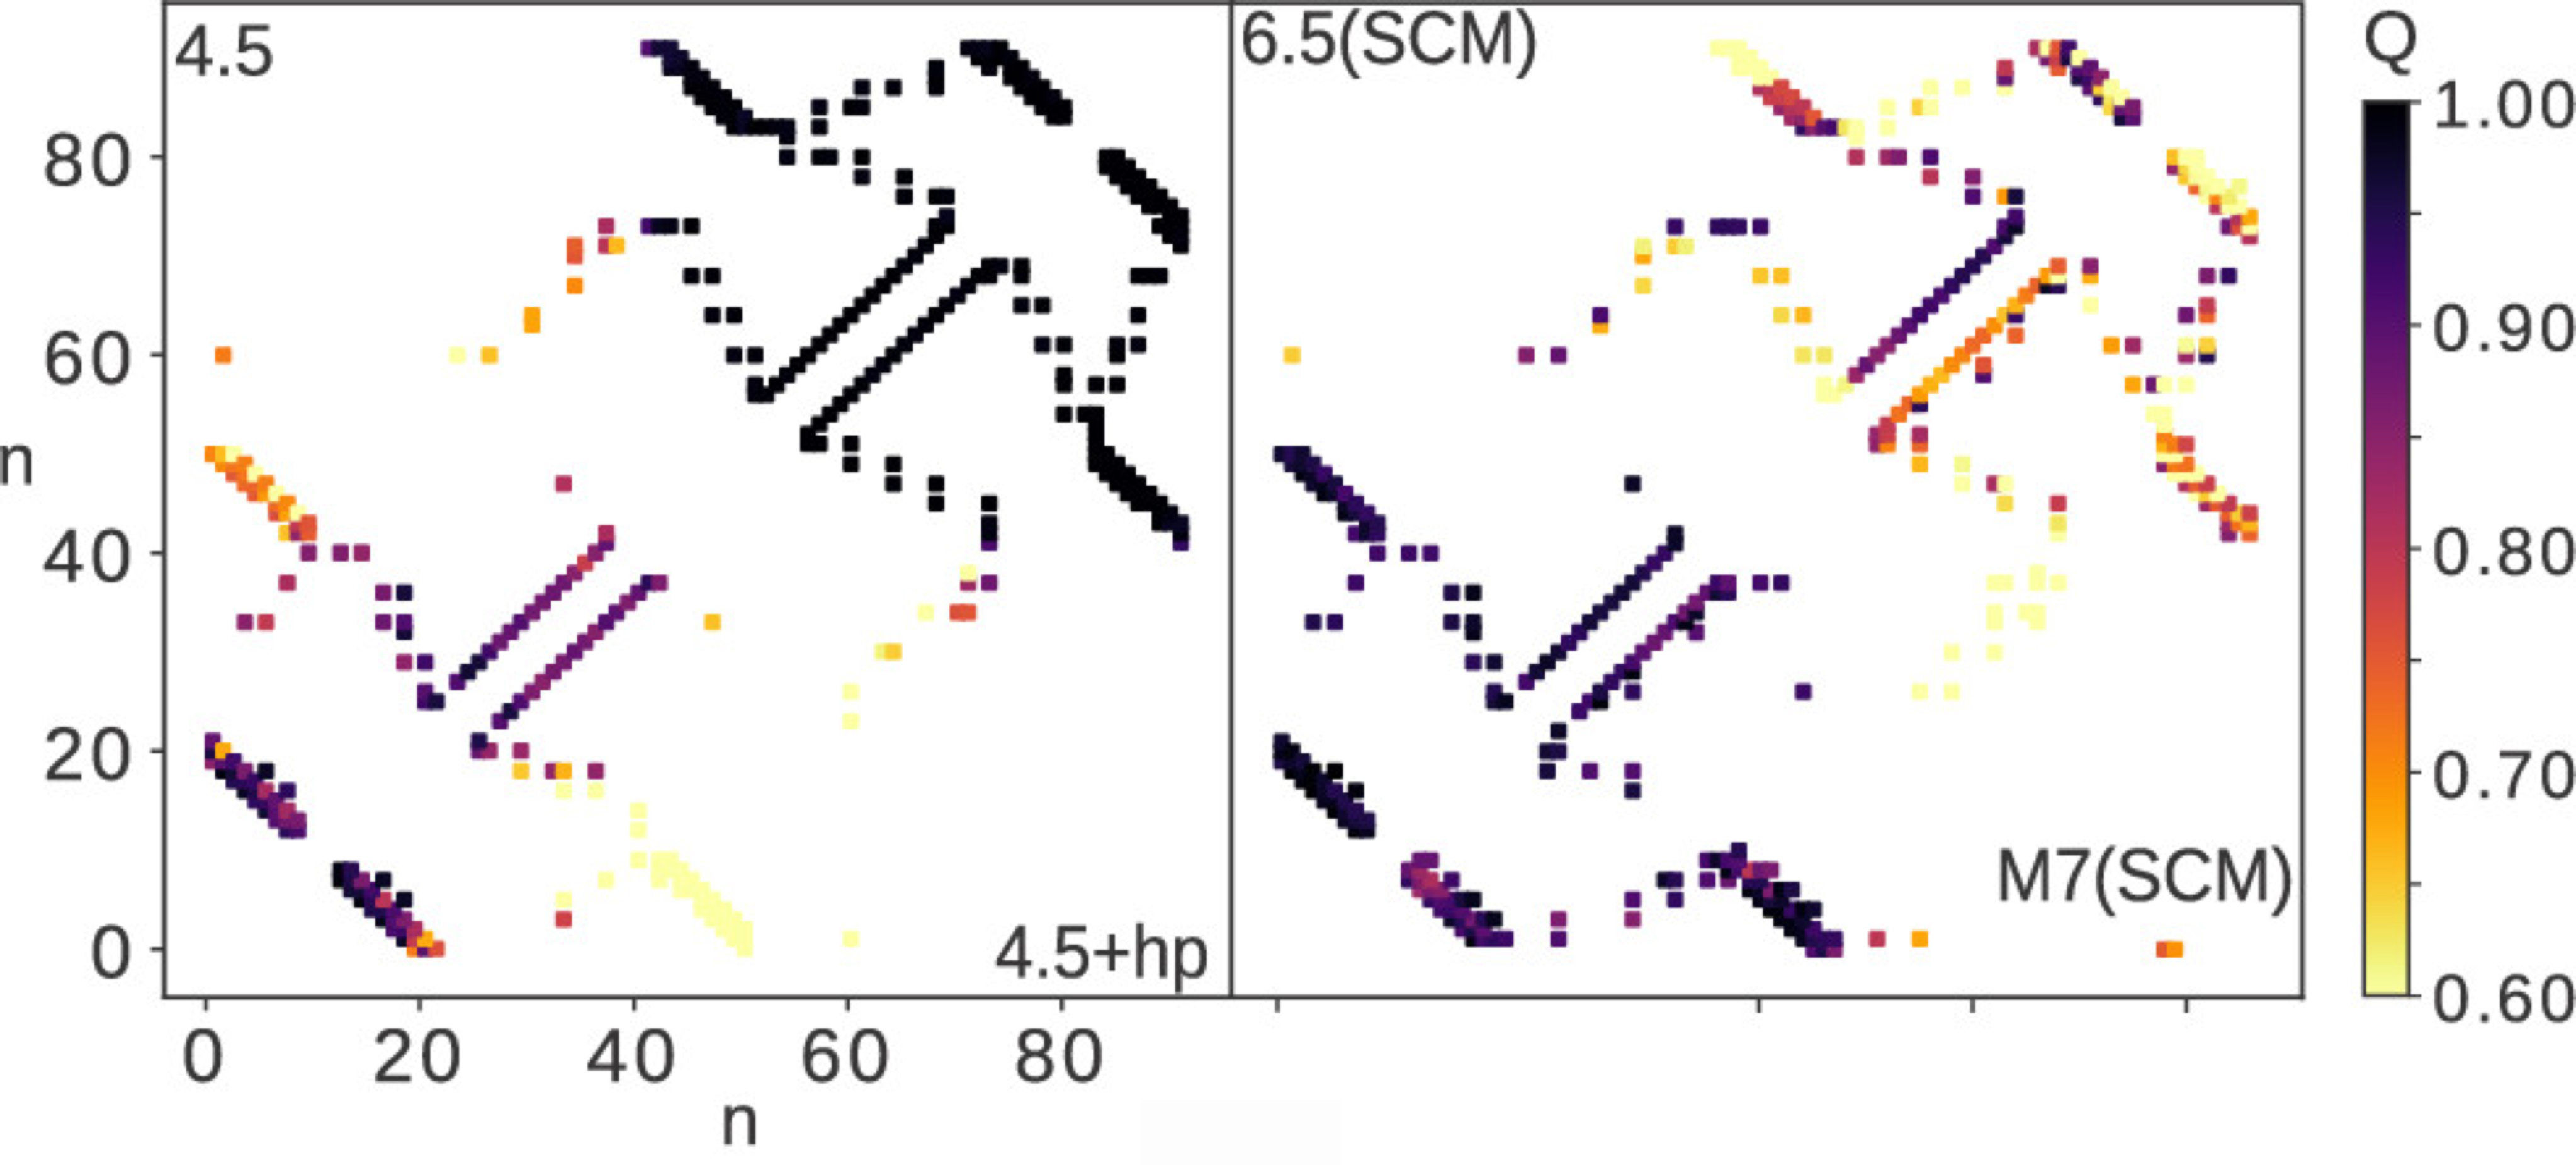
\includegraphics[width=\linewidth]{pcmap.pdf}
\end{center}
\vspace{-0.4cm}
Four separate contact maps depicting the probability of formation of each contact in the ensemble of minima found from DPS. Addition of hydrophobic interactions destabilises the N-terminal region considerably. The SCM method changes the folding route of Top7 making unfolding from the C-terminal more favourable. 
}
\headerbox{7. MJ0366: A simple trefoil knot}{name=MJ0366,column=2, span=1, below=PCM}{

\begin{center}
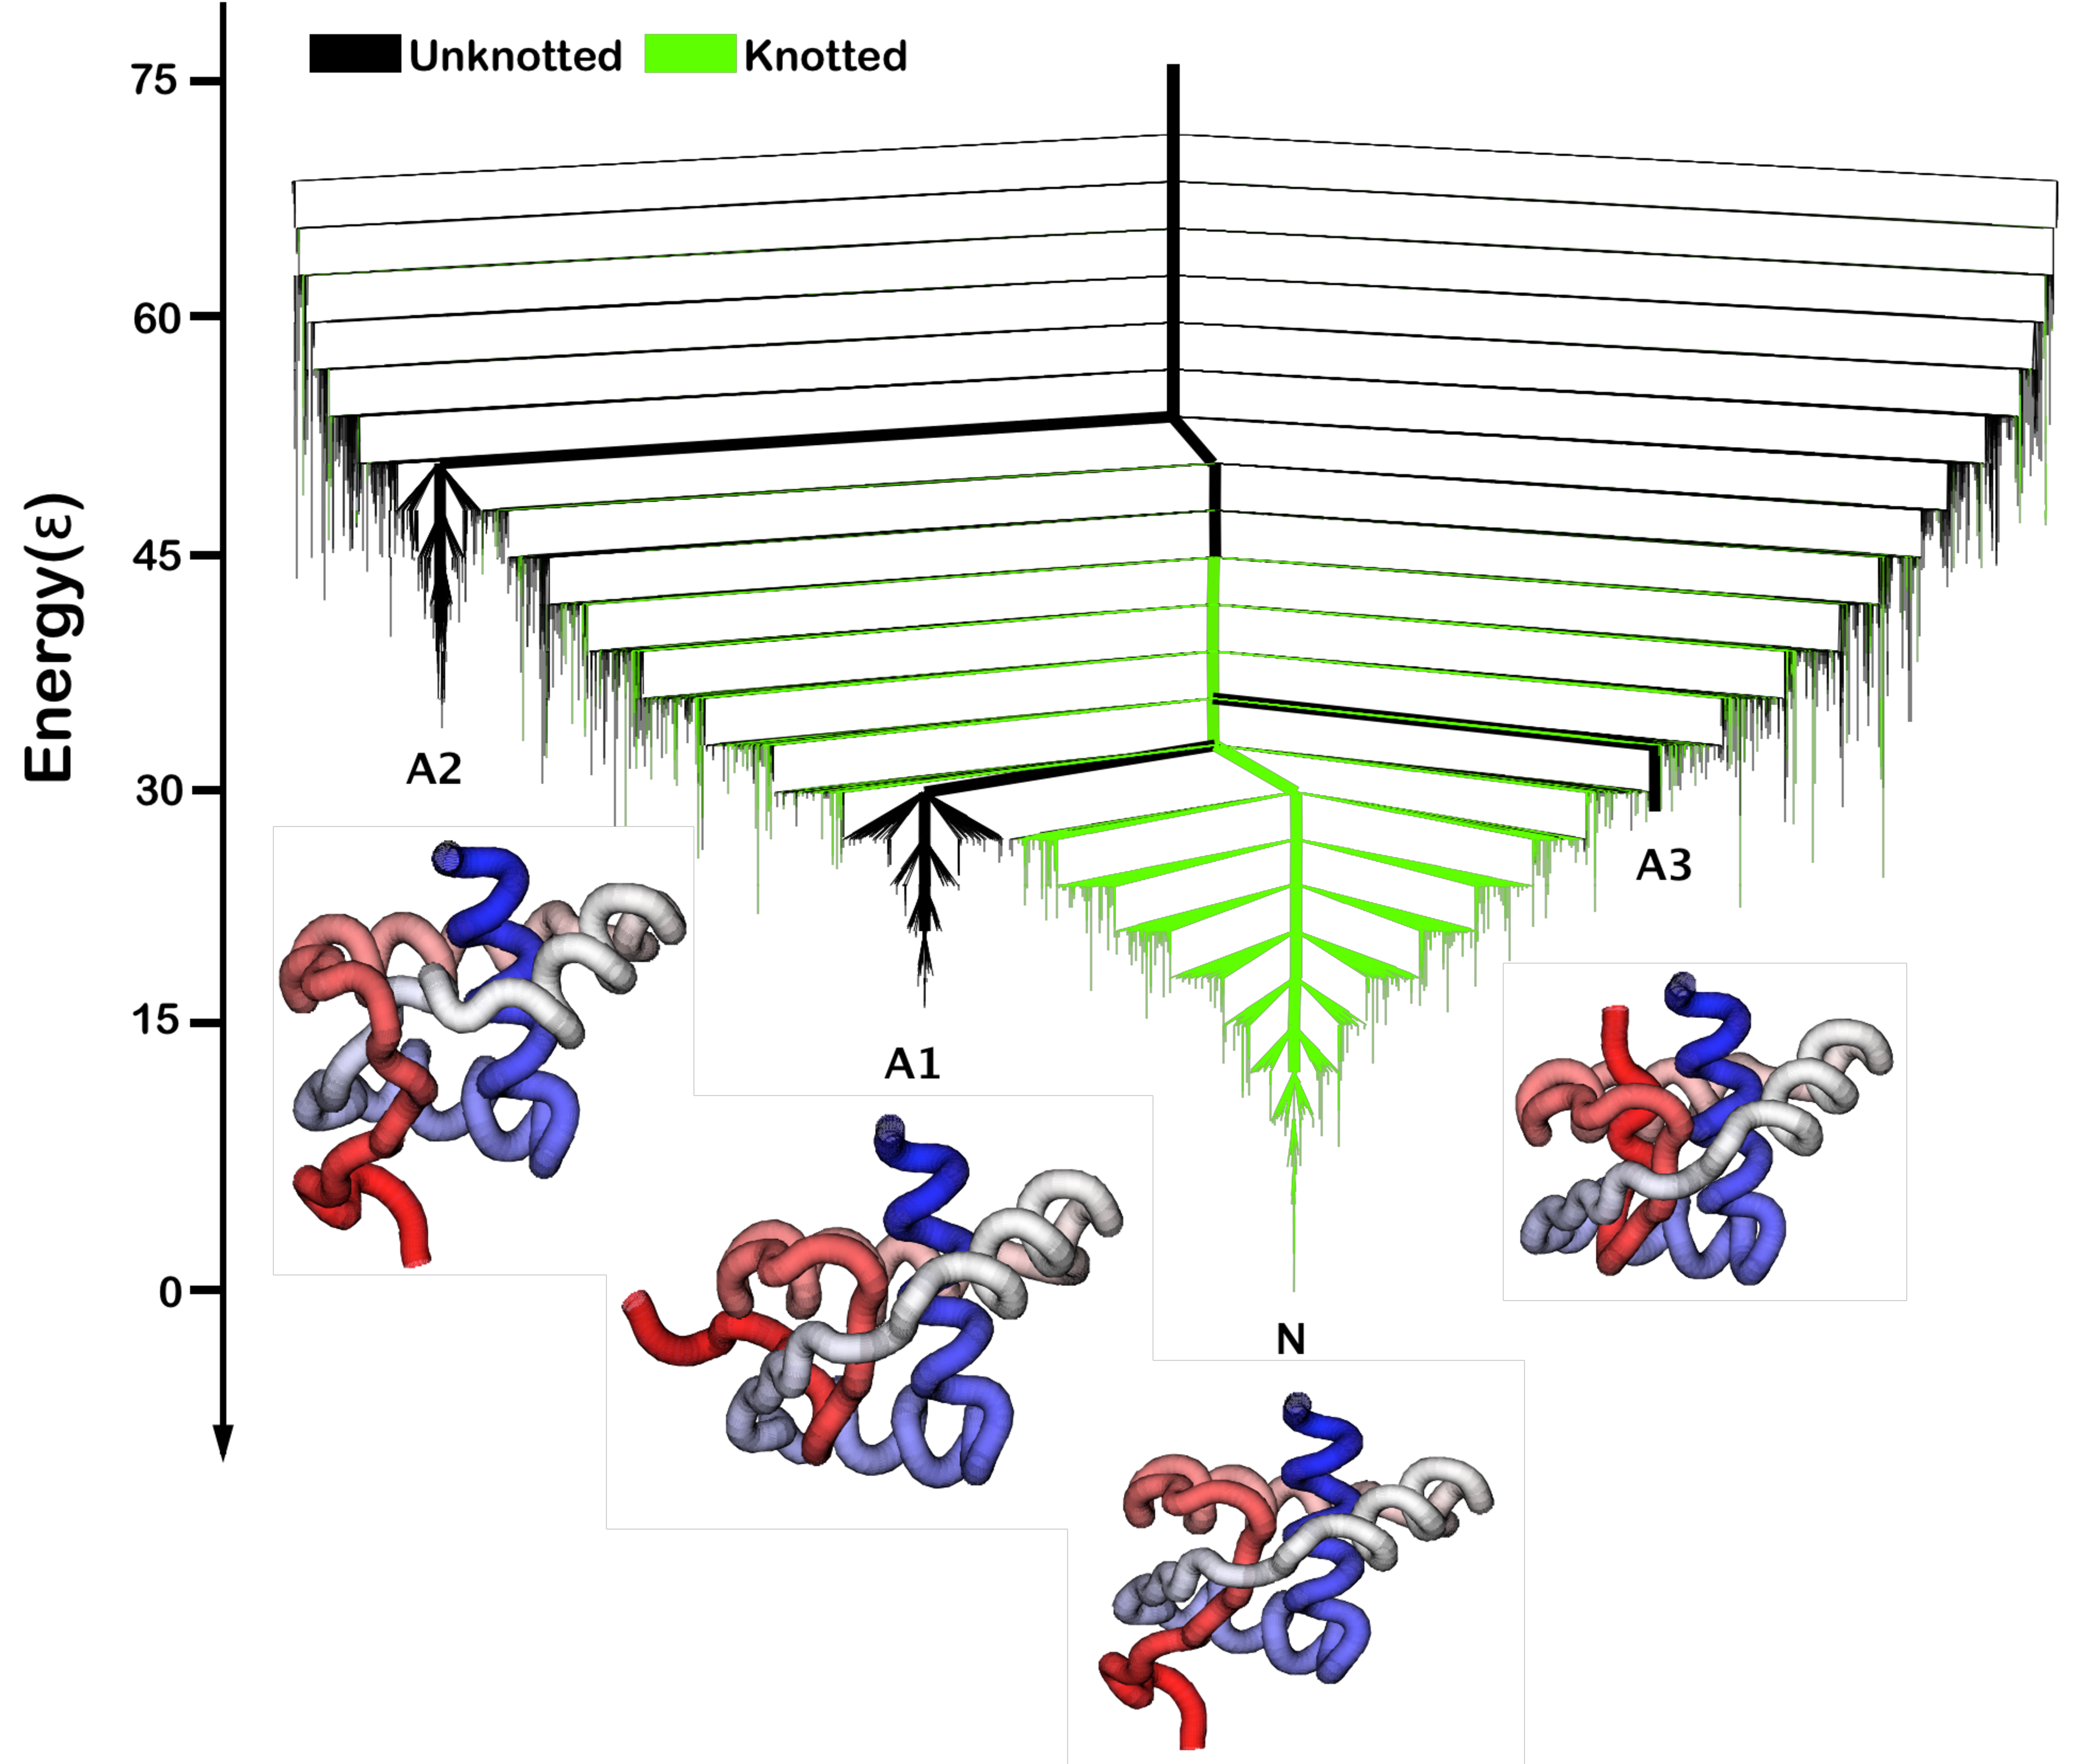
\includegraphics[width=0.7\linewidth]{MJ0366.pdf} 
\end{center}
\vspace{-0.5cm}
Disconnectivity graph representation of a trefoil knotted protein. In keeping with literature [6], structures A1, A2 and A3 were identified as topological traps. Both slip-knotting and plugging mechanisms are observed (See video). First threading event proceeds from the N-terminal. ``Backtracking'' proceeds from the A1 and A2  basins. 
}

\headerbox{8.HI0766: A shallow and a deep trefoil knot}{name=HI0766,column=0, span=2, below=Top7DPS}{
\begin{multicols}{2}
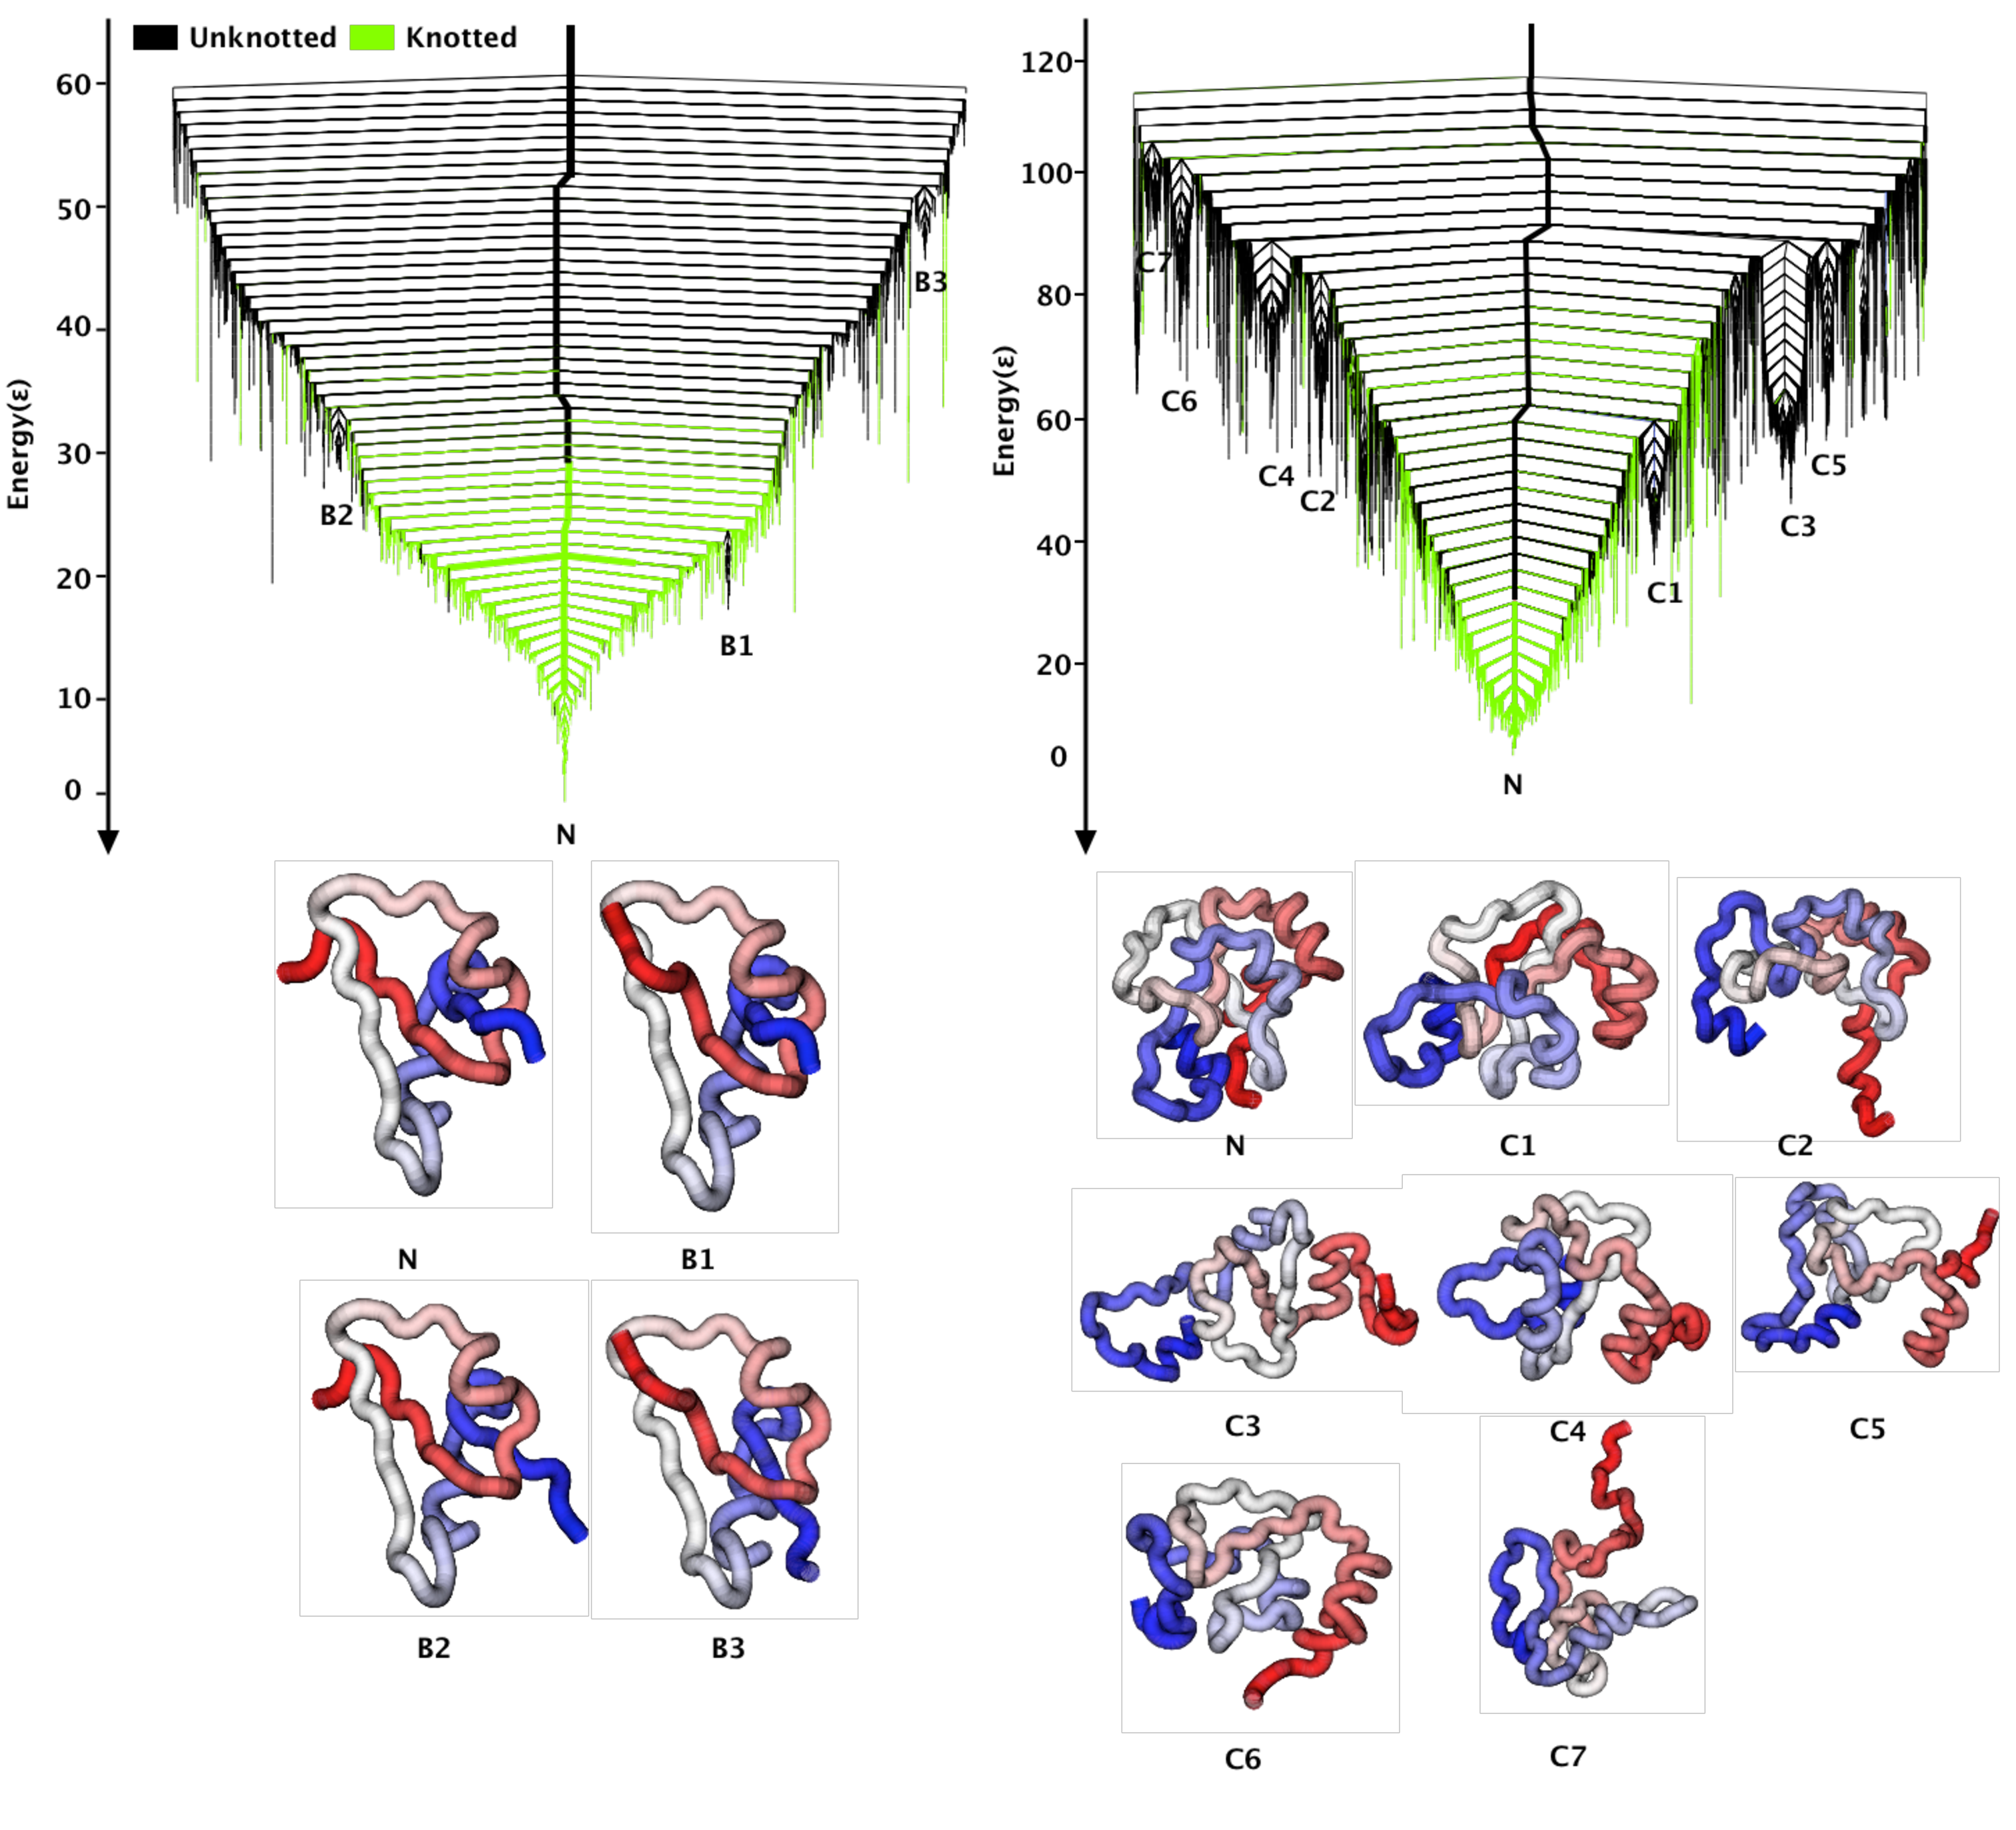
\includegraphics[width=\linewidth,]{all.pdf}
N-terminal in red and C-terminal in blue. Nodes in green indicate the structure is a 3$_1$ knot. 
\columnbreak
\begin{itemize}
    \item {Disconnectivity graph representation of a shallow trefoil knot (left) and a deep trefoil knot (right) for the protein HI0766 (YibK,PDBID:1mxi). A shallow knot is defined as one containing 5 residues on either side of the knotted region while a deep knot contains 20 residues on either side of the knotted region. PEL for the deep knot is more frustrated than that of the shallow knot. }
    \item{\vspace{-0.5cm}Each minimum is classified as a knot or an unknot. Knotting begins $\approx$30$\varepsilon$ above the native-state. Low-energy unknotted basins result in the ``backtracking'' mechanism. Multiple pathways leading to the knotted state are observed (See video). Threading proceeds from the C-terminal as observed in experiment. }
    %\item{Traps obtained from DPS are depicted below the disconnectivity graphs. Colouring is identical to section 7.}
\end{itemize}
\end{multicols}
}%

\headerbox{References}
{name=references,column=2,span=1,below=MJ0366}{
\small
\renewcommand*{\bibfont}{\footnotesize}
\renewcommand*{\bibfont}{\footnotesize}
\bibfont{\textbf{1.} D. J. Wales, Mol. Phys. 100, 3285 (2002),} 
\bibfont{\textbf{2.} Neelamraju et al, J. Phys. Chem. B 122,51,12282-12291 (2018),} 
\bibfont{\textbf{3.} Neelamraju et al, J. Chem. Inf.  Model., 59, 5, 1703-1708 (2019),}
\bibfont{\textbf{4.} O. M. Becker and M. Karplus, J. Chem. Phys. 106, 1495 (1997),}
\bibfont{\textbf{5.} Truong et al, J. Chem. Phys. 139,12, 121908 (2013), \textbf{6.} Noel et al, Proc. Nat. Acad. Sci., 107,35,15403-15408 (2010)}
}
% \renewcommand{\bibsection}{}
% \bibliography{poster}
% \bibliographystyle{plain}
% %\nocite{*} % Insert publications even if they are not cited in the poster
% [1] Liu and Chan, J. Mol. Biol. 349(4);872-889, 2005.[2] Cheung and Onuchic, J. Phys. Chem. B, 107(40):11193-11200,2003. [3] http://www-wales.ch.cam.ac.uk/PATHSAMPLE.[4] Becker and Karplus. J. Chem. Phys.,106(4):1495-1517,1997.,[5] Truong and Wolynes,J. Chem. Phys 139(12):121908,2013.



\end{poster}

\end{document}
